% Begin of the presentation
\documentclass{beamer}
\usetheme{LEA}
\usepackage{hyperref}
\usepackage{pgf}
\usepackage[utf8]{inputenc}
\usepackage{amsmath}
\usepackage{amsfonts}
\usepackage{amssymb}
\usepackage{amsthm}
\usepackage{graphicx}
%\usepackage[shortend]{algorithm2e}
%\usepackage{multicol}
%\usepackage{tikz}
\usepackage{csquotes}
\usepackage[ngerman]{babel}

\usepackage{bbding}


\definecolor{light-gray}{gray}{0.95}
\definecolor{DarkGrey}{rgb}{0.1,0.1,0.1}

%other header tings I did
\usepackage{listings}
\lstset{% general command to set parameter(s)
basicstyle=\footnotesize\color{black}, % print whole listing small
backgroundcolor=\color{light-gray},
numbers=none,
captionpos=b,
tabsize=4,
breaklines=true,
frame=single,
keywordstyle=\color{violet}\bfseries,
commentstyle=\color{DarkGrey},
stringstyle=\color{blue},
showstringspaces=false,
basicstyle=\small
}




%entfernen der Navigationsleiste
\beamertemplatenavigationsymbolsempty

%                                 PDF information fields
%\hypersetup{
%	pdftitle={Mathematik der Wahlverfahren},
%	pdfauthor={Corelius Diekmann},
%	pdfsubject={Seminar Wissenschaftler und Ethik -- Winter 11/12},
%	pdfcreator=pdflatex,
%	pdfproducer=pdflatex,
%	pdfnewwindow=true,
%	pdfpagemode=FullScreen,
%	pdfview=FitBH,
%	plainpages=false,
%	baseurl={./}
%}

%                          Information for the Title Page
%
\title[Mathematik der Wahlverfahren]{
	\Large Mathematik der Wahlverfahren\\
	[5mm] \normalsize Seminar Wissenschaftler und Ethik \\
	Winter 11/12
}
\author{Cornelius Diekmann}
\institute[]{
	Fakult\"at f\"ur Informatik\\
	TU M\"unchen\\[3mm]
}
\date{\today}
%\titlegraphic{% 
%	\vspace{5mm}%
%	\includegraphics[height=7mm]{fau_logo}%
%	\hspace{10mm}%
%	\includegraphics[height=7mm]{tum_logo}%
%	\hspace{10mm}%
%	\includegraphics[height=7mm]{stuttgart_logo}%
%}


%                                Beginning of the document 
%
\begin{document}

\begin{frame}
	\titlepage
\end{frame}

\begin{frame}
	\frametitle{Inhalt}
	\tableofcontents
\end{frame}

\section{Einführung}
\subsection{Theorie der Wahlsysteme}
\begin{frame}[fragile]
	\frametitle{Einführung}
	Theorie der Wahlsysteme
	\begin{itemize}
		\item gegeben: individuelle Meinungen der Wähler
		\item gesucht: Kollektiventscheidung
		\pause
		\item Randbedingungen
		\begin{itemize}
			\item fair
			\item demokratisch
			\item sicher vor Betrug
			\item gibt den Willen der Wähler wieder
			\item ...
		\end{itemize}
	\end{itemize}
\end{frame}

\subsection{Aktuelles Beispiel}
\begin{frame}[fragile]
	\frametitle{Beispiel Deutschland}
	\begin{columns}
		\begin{column}[t]{0.6\textwidth}
				\begin{block}{Deutsches Wahlrecht (vereinfacht)}
				
				\begin{itemize}
					\item 2x eine Stimme
					\item Erststimme: Kandidat
					\item Zweitstimme: Partei
					\item Mehrheitsentscheid
				\end{itemize}
					
				\end{block}
			\end{column}
			\begin{column}[t]{0.4\textwidth}
				\begin{block}
				
				%\begin{figure}[!htb]
				%\begin{center}
				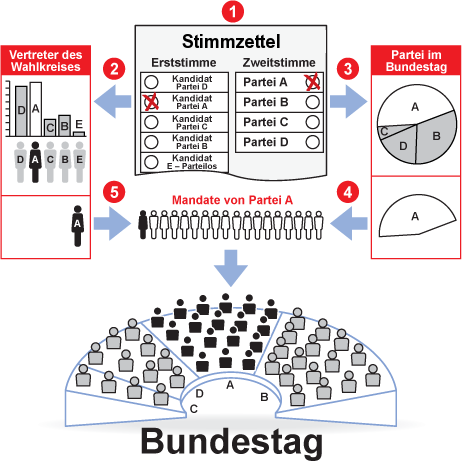
\includegraphics[width=\linewidth]{Pers-Ver-Wahl-v4}
				%\end{center}
				%\caption{}
				%\end{figure}
				
				\footnotesize{Quelle: \cite{imgdtwahl}}
				
				
				\end{block}
			\end{column}
		\end{columns}
\end{frame}



\begin{frame}[fragile]
	\frametitle{Beispiel Deutschland}
	
	Deutsches Wahlrecht verfassungswidrig
	\begin{itemize}
		\item Bundesverfassungsgericht 2008\footnote{Az.: 2 BvC 1/07, \cite{handelsblattverf, spiegelverf}}
		\item negatives Stimmgewicht
	\end{itemize}

	%\begin{figure}[!htb]
	\begin{center}
	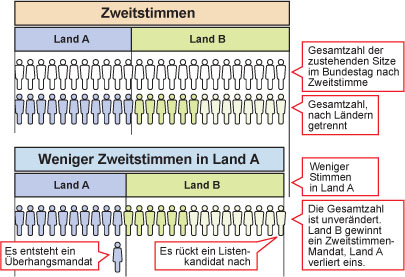
\includegraphics[width=0.5\linewidth]{Neg-Simmen-Gewicht3}\footnote{Quelle: \cite{imgnegstim}}
	\end{center}
	%\caption{}
	%\end{figure}
\end{frame}

\section{Wahlverfahren mathematisch}
\begin{frame}[fragile]
	\frametitle{Wahlverfahren formal \cite{hodge2005mathematics, bungartz}}
	
	\begin{itemize}
		\item Kandidaten $A, B, C, ...$
		\item Präferenzen $ A \succ B $, $ A \succeq B$
		\pause
		\item Rangordnung $ B \succ A \succ C \succ P \succeq X \succeq Y \succeq Z \succ N $
		\begin{itemize}
			\item Transitivität
		\end{itemize}
		\pause
		\item Betrachtung der kompletten Wählerpräferenzen
		\pause
		\begin{itemize}
			\item kompletten Wählerpräferenzen für theoretische Diskussion notwendig $\Rightarrow$ Kompromisse
			\item Deutschland: nur erster Platz; nur 1 Kandidat
			\item Australien und Irland: Angabe kompletter Rangliste möglich \cite{spektrum}
		\end{itemize}
	\end{itemize}
	\pause
	Wahlverfahren: 
	$$ \left\{ x | x \ \mathrm{totale\ Ordnung} \right\} ^{|\mathrm{W"ahler}|} \rightarrow \left\{ x | x \ \mathrm{totale\ Ordnung} \right\}$$

\end{frame}

\section{Wünschenswerte Eigenschaften}
\begin{frame}[fragile]
	\frametitle{Wünschenswerte Eigenschaften}
	Bis jetzt:
	\pause
	\begin{itemize}
		\item innerer Diktator?
		\pause
		\item konstante Funktion?
		\pause
		\item negatives Stimmgewicht
		\pause
	\end{itemize}
	\begin{definition}
	Ein Wahlverfahren heißt \emph{monoton} g.d.w sich eine Individualentscheidung zum Vorteil eines Kandidaten im Gesamtergebnis nicht negativ auf diesen Kandidaten auswirken kann.
	\end{definition}
\end{frame}


\begin{frame}[fragile]
	\frametitle{dt. Grundgesetz}
	\begin{quote}
	\textit{Die Abgeordneten des Deutschen Bundestages werden in allgemeiner, unmittelbarer, freier, gleicher und geheimer Wahl gewählt.} \cite{ggwahlrecht}
	\end{quote}
	\pause
	\begin{definition}
	Ein Wahlsystem heißt \emph{anonym}, g.d.w es jeden Wähler gleich behandelt.
	\end{definition}
	\begin{definition}
	Ein Wahlsystem heißt \emph{neutral}, g.d.w es jeden Kandidaten gleich behandelt.
	\end{definition}
\end{frame}


\section{Wahlverfahren im Vergleich}
\begin{frame}[fragile]
	\frametitle{Absolute Mehrheit}
	\begin{itemize}
		\item Sieger: mehr als $50\%$ der 1. Plätze
		\pause
		\item ernennt eindeutigen Sieger bei $\leq 2$ Kandidaten
		\pause
		\item monoton, neutral, anonym
		\pause
		\item keine Paradoxien
		\pause
		\item fair (?)
		\pause
		\item einzig sinnvolles demokratisches Verfahren für zwei Kandidaten, May's Theorem \cite{hodge2005mathematics}
	\end{itemize}
\end{frame}

\begin{frame}[fragile]
	\frametitle{Relative Mehrheit}
	\begin{itemize}
		\item Sieger: Kandidat mit meisten Erstplatzierungen
		\pause
		\item monoton, neutral, anonym
		\pause
		\item absolute Mehrheitsbedingung
		\pause
		\item keine Paradoxien?
	\end{itemize}
	\pause
	\begin{table}[h]
	\centering
	\begin{tabular}{c|c}
	Stimmen & Präferenzen \\
	\hline
	35 & $ N \succ S \succ J $\\ 
	28 & $ S \succ N \succ J $ \\
	20 & $ J \succ N \succ S $ \\
	17 & $ J \succ S \succ N $ \\
	\end{tabular}
		\caption{Zahlen angelehnt an die Wahl des Wrestlers Jesse Ventura 1998 zum Governor in Minnesota. Quelle \cite[Table 3.1]{hodge2005mathematics}.}
		\label{tab:wrestlerwahl}
	\end{table}
\end{frame}


\begin{frame}[fragile]
	\frametitle{Borda Methode}
	\begin{definition}
	Für eine Wahl mit $n$ Kandidaten werden Punkte für jeden Kandidaten errechnet:
	\begin{itemize}
	\item Jede Erstplatzierung schreibt dem Kandidaten $n-1$ Punkte zu
	\item Jede Zweitplatzierung schreibt dem Kandidaten $n-2$ Punkte zu
	\item $\cdots$
	\item Jeder letzte Platz wird mit $0$ Punkten gewertet
	\end{itemize}
	Die resultierende Rangordnung ist die Liste der Kandidaten geordnet nach der Anzahl der erworbenen Punkte.
	\end{definition}
\end{frame}

\begin{frame}[fragile]
	\frametitle{Borda Methode}

	\begin{table}[h]
	\centering
	\begin{tabular}{c|c}
	Stimmen & Präferenzen \\
	\hline
	35 & $ N \succ S \succ J $\\ 
	28 & $ S \succ N \succ J $ \\
	20 & $ J \succ N \succ S $ \\
	17 & $ J \succ S \succ N $ \\
	\end{tabular}
	\end{table}
	
	\begin{itemize}
		\item $N$ $118$ Punkte
		\item $S$ $108$ Punkte
		\item $J$ $74$ Punkte
		\item $ N \succ S \succ J $
		\pause
		\item aber: verletzt absolutes Mehrheitskritrium
	\end{itemize}
\end{frame}

\begin{frame}[fragile]
	\frametitle{Condorcet Gewinner Kriterium}

	\begin{definition}
		Als Condorcet Gewinner wird ein Kandidat bezeichnet, der in jedem Zweikampf (ausgetragen mit absolutem Mehrheitsentscheid) gewinnen würde.
		
		Ein Wahlsystem erfüllt das Condorcet Gewinner Kriterium falls ein Condorcet Gewinner stets die Wahl gewinnt -- falls einer existiert.
	\end{definition}
	
	Erfüllt durch:
	\pause
	\begin{itemize}
		\item Absolute Mehrheit ? \pause \Checkmark \pause
		\item Relative Mehrheit ? \pause \XSolidBrush \pause
		\item Borda Methode ? \pause \XSolidBrush
	\end{itemize}
\end{frame}


\begin{frame}[fragile]
	\frametitle{Sequential Pairwise Voting}
	\begin{itemize}
		\item Idee: Spalte in Mehrheitsentscheide auf -- Zweikampf
				
	
		\begin{columns}
				\begin{column}[t]{0.6\textwidth}
						\begin{block}{}
						\begin{itemize}
							\item Erfüllt Condorcet Gewinner Kriterium
							\item Monoton
							\item Absolutes Mehrheitskritrium
							\item neutral?
						\end{itemize}
						\end{block}
					\end{column}
					\begin{column}[t]{0.4\textwidth}
						\begin{block}
						
						\begin{tikzpicture}[>=latex']
						    \tikzstyle{every node}=[circle,draw]
						    \node {\_}
						        child { node {D} }
						        child {
						        	            node {\_}
						        	            child { node {C} }
						        	            child {
						        	            	            node {\_}
						        	            	            child { node {B} }
						        	            	            child { node {A} }
						        	            	        }
						        	        }
						    ;
						\end{tikzpicture}
						
						
						\end{block}
					\end{column}
		\end{columns}
	\end{itemize}
	
\end{frame}


\subsection{Zusammenfassung}
\begin{frame}[fragile]
	\frametitle{Zusammenfassung}

	\centering
	\begin{tabular} {c |  *{6}{p{0.1\textwidth}|}}%{c|p|p|p|p|p}
	Wahlsystem & Anonym & Neut. & Mono. & AM & CG \\
	\hline
	Absolute Mehrheit & \Checkmark & \Checkmark & \Checkmark & \Checkmark  & \Checkmark \\ 
	Relative Mehrheit & \Checkmark & \Checkmark & \Checkmark & \Checkmark  & \XSolidBrush \\ 
	Borda Methode & \Checkmark & \Checkmark & \Checkmark & \XSolidBrush  & \XSolidBrush \\ 
	Sequential Pairwise Voting & \Checkmark & \XSolidBrush & \Checkmark & \Checkmark  & \Checkmark \\ 
	\end{tabular}
\end{frame}

\section{Aktive Wahlmanipulation}
\begin{frame}[fragile]
	\frametitle{Aktive Wahlmanipulation}
	\begin{itemize}
		\item durch Wahlfälschung
		\item durch mathematischen Schwächen
	\end{itemize}
	\pause
	Beispiel:
	\begin{itemize}
		\item Bundestagsnachwahl Dresden 2005
		\item CDU Wähleraufklärung
		\item \emph{weniger} als $41 225$ Zweitstimmen gewünscht
		\item sonst Mandatverlust durch negatives Stimmgewicht
	\end{itemize}
	\pause
	Mehrheitsentscheid:
	\begin{itemize}
		\item schwäche Ideologie durch neun Kandidaten dieser Ideologie
		\pause
		\item Stimmen für diese Ideologie teilen sich auf Kandidaten auf
	\end{itemize}
	\pause
	Borda Methode:
	\begin{itemize}
		\item mehr Kandidaten für eine Ideologie
		\pause
		\item taktisches Wählen: setzte Konkurrenten des Wunschkandidaten an letzte Stelle
	\end{itemize}
\end{frame}


\begin{frame}[fragile]
	\frametitle{Unabhängigkeit irrelevanter Alternativen}
	Manipulation wie folgt erkennen:
	\begin{itemize}
		\item Ergebnis der Wahl $A \succ B$
		\item Wahl wiederholen
		\item alle Wähler behalten ihre Meinung bezüglich $A$ und $B$
		\pause
		\item $\Rightarrow$ Endergebnis bezüglich $A$ und $B$ darf sich nicht ändern
	\end{itemize}
\end{frame}


\section{Arrow's Unmöglichkeitssatz}
\begin{frame}[fragile]
	\frametitle{Arrow's Unmöglichkeitssatz}
	\begin{enumerate}
		\item \label{a-1} Wahlsystem: $ \left\{ x | x \ \mathrm{totale\ Ordnung} \right\} ^{|\mathrm{W"ahler}|} \rightarrow \left\{ x | x \ \mathrm{totale\ Ordnung} \right\}$
		\item \label{a-w-i} Alle transitiven Individualentscheidungen müssen zulässig sein.
		\item \label{a-3} Wenn alle (!!) Wähler $A \succ B$ wählen, muss auch in der Kollektivrangliste $A \succ B$ gelten.
		\item \label{a-4} Die Unabhängigkeit irrelevanter Alternativen gilt.
	\end{enumerate}
	\pause
	$\Rightarrow$ Im resultierenden Wahlsystem gibt es einen Wähler, dessen Individualpräferenzen eins zu eins als Kollektiventscheidung übernommen werden.
\end{frame}


\begin{frame}[fragile]
	\frametitle{Diskussion}
	\begin{itemize}
		\item Verletzung der Anonymitätsbedingung
		\pause
		\item nicht manipulierbares System das jedem Wähler die Freiheit lässt seine Meinung frei zu äußern, ähnelt im Gesamtergebnis der Wahl einer Diktatur
		\pause
		\item existieren Kompromisslösungen im Allgemeinen?
		\pause
		\item mathematisches Problem oder ethisches?
	\end{itemize}
\end{frame}


\section{Wahlverfahren die Arrow meiden}
\begin{frame}[fragile]
	\frametitle{Approval Voting}
	\begin{itemize}
		\item Idee: verletzte  Arrow's Bedingung \ref{a-w-i}
	\end{itemize}
	\begin{definition}
	Jeder Wähler erstellt eine Rangordnung. In dieser Rangordnung muss ``$\succ$'' genau einmal vorkommen. Der Gewinner wird per relativen Mehrheitsentscheid festgestellt.
	\end{definition}
\end{frame}

\begin{frame}[fragile]
	\begin{center}
		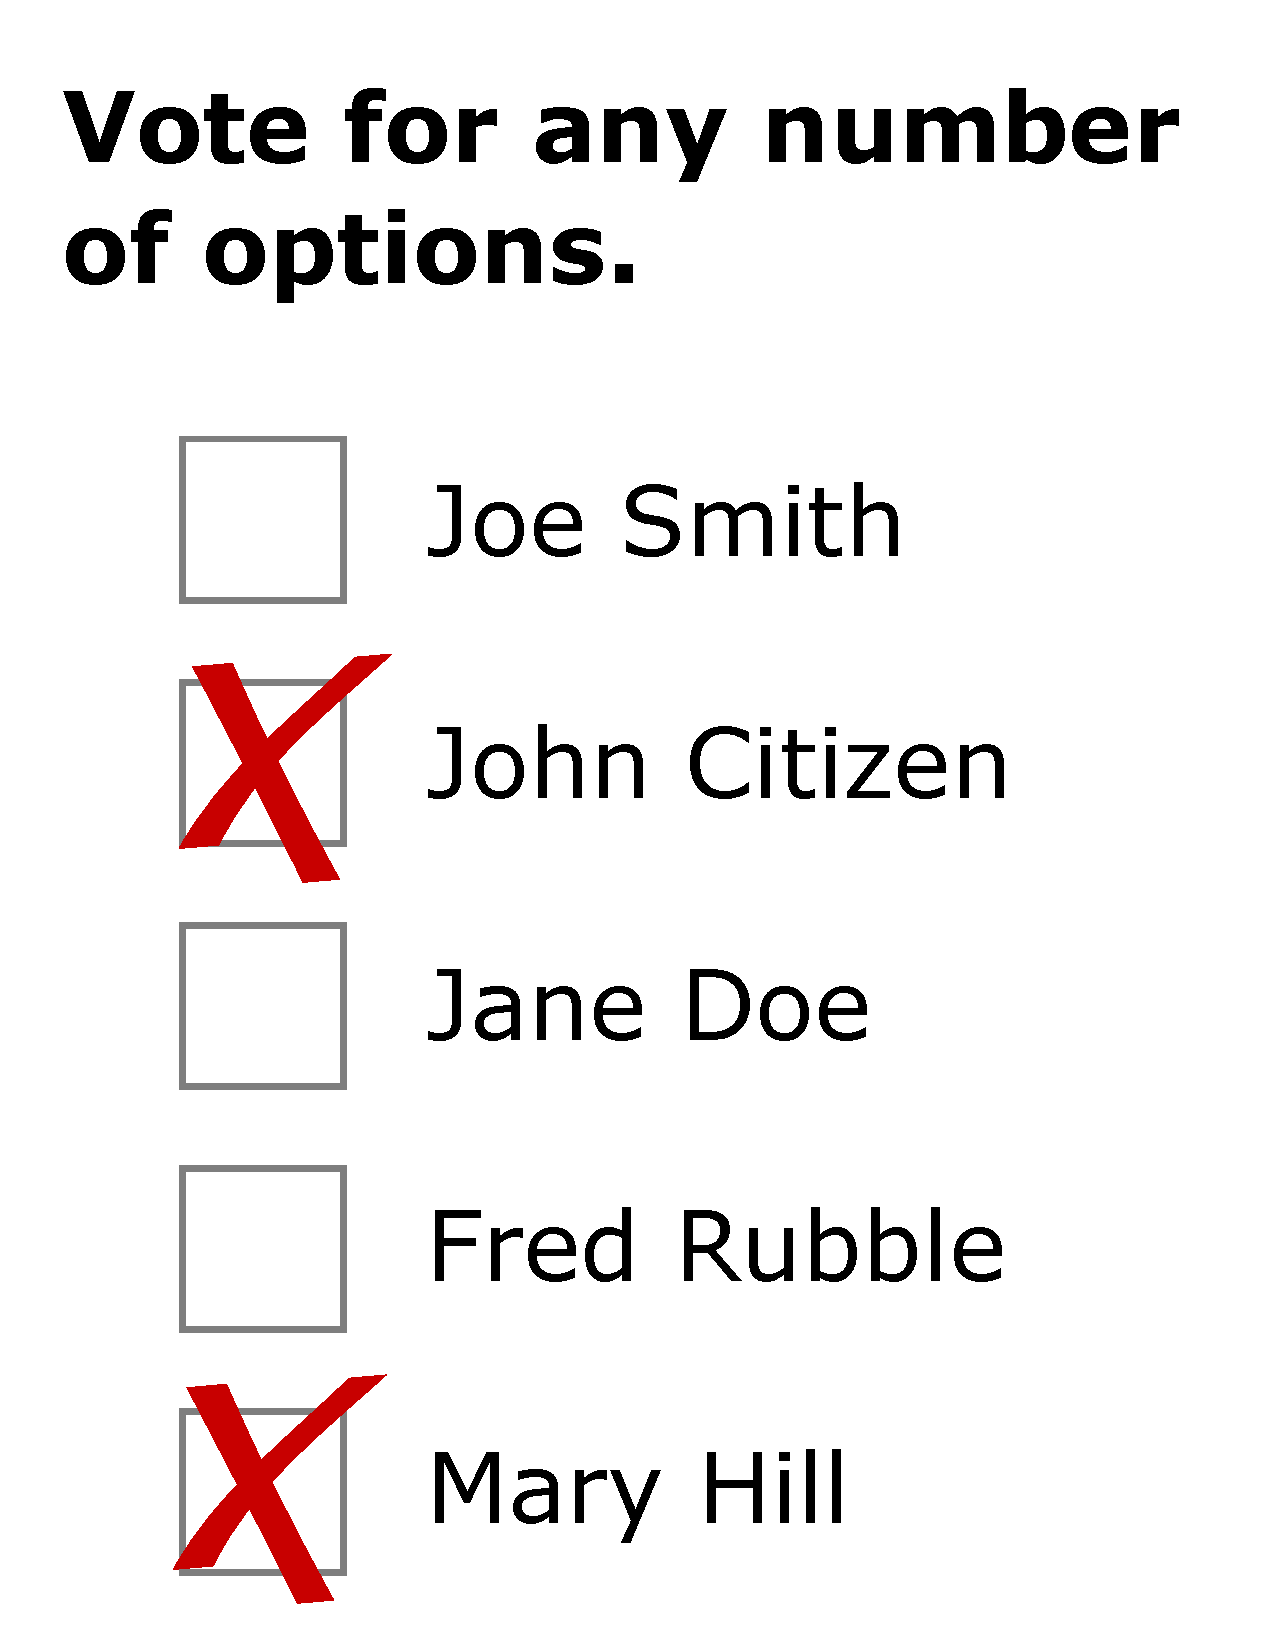
\includegraphics[width=0.5\linewidth]{approval-ballot.pdf}\footnote{Quelle: \cite{apprwiki}}
	\end{center}
\end{frame}


\section{Quellen}
\begin{frame}
	%\bibliographystyle{alpha}  % try `plain' or 'abbrv' instead of 'alpha'
	%\bibliography{paper} % references are in the file "paper.bib"
	\bibliographystyle{IEEEtran} % IEEE cite fuck yeah
	\begin{tiny}
		\bibliography{../paper/paper} % references are in the file "paper.bib"
	
	\end{tiny}
\end{frame}


\begin{frame}
	\begin{center}
		Thank you!
	\end{center}
\end{frame}
\end{document}
